In this section, we describe the plugin-based architecture of our framework, designed to systematically 
collect, standardize, and preprocess anatomical MRI data. We discuss its modular structure by explaining 
the functions and interdependencies of each module.


\subsection{Overall Framework Design}

Our framework is developed in Python and employs a configurable plugin-based architecture to allow flexible 
substitution of plugins without the need for updating the codebase. Each module, 
or plugin, is responsible for a specific task, such as downloading MRI data from a given repository, 
performing MRI preprocessing, or mapping the downloaded files to a standardized JSON record (Figure~\ref{fig:SystemArchitecture}).
This design allows researchers to easily swap out or introduce new plugins (e.g., new preprocessing pipelines) customized to meet their specific research needs.
Key objectives of the framework include: 
\begin{description}
    \item[Automation:] Minimizing manual labor by automating dataset downloads, file mapping and organization, demographics attachment, and data preprocessing in a single pipeline.
    \item[Standardization:] Maintaining a common mapping record and a standardized preprocessing pipeline across all datasets, while allowing users the flexibility to incorporate dataset-specific preprocessing or other customized plugins as needed.
    \item[Extensibility:] Facilitating seamless integration of new data sources, additional preprocessing pipelines, and integration of new modules or plugins. 
    \item[Reproducibility:] Ensuring consistent execution and traceability by recording dataset-specific download, mapping, and processing parameters in JSON configuration files, thus facilitating accurate and reliable replication of the workflow.
\end{description}


\subsection{Plugin-Based Architecture}

Figure~\ref{fig:SystemArchitecture} illustrates the framework architecture of BrainScape. 
At the core of this framework is a pipeline workflow that handles the sequential execution of the modules, 
such as downloading, mapping, and preprocessing (depicted by the red arrows in Figure~\ref{fig:SystemArchitecture}). 
This framework allows flexible selection and configuration of the plugins for each step, which can be tailored for 
each individual dataset via dataset-specific configuration files.
The Configurations integrate both default settings and dataset-specific overrides, maintaining consistency 
across datasets while allowing the flexibility to individually customize the pipeline for each dataset.

\begin{figure}[htbp]\begin{center}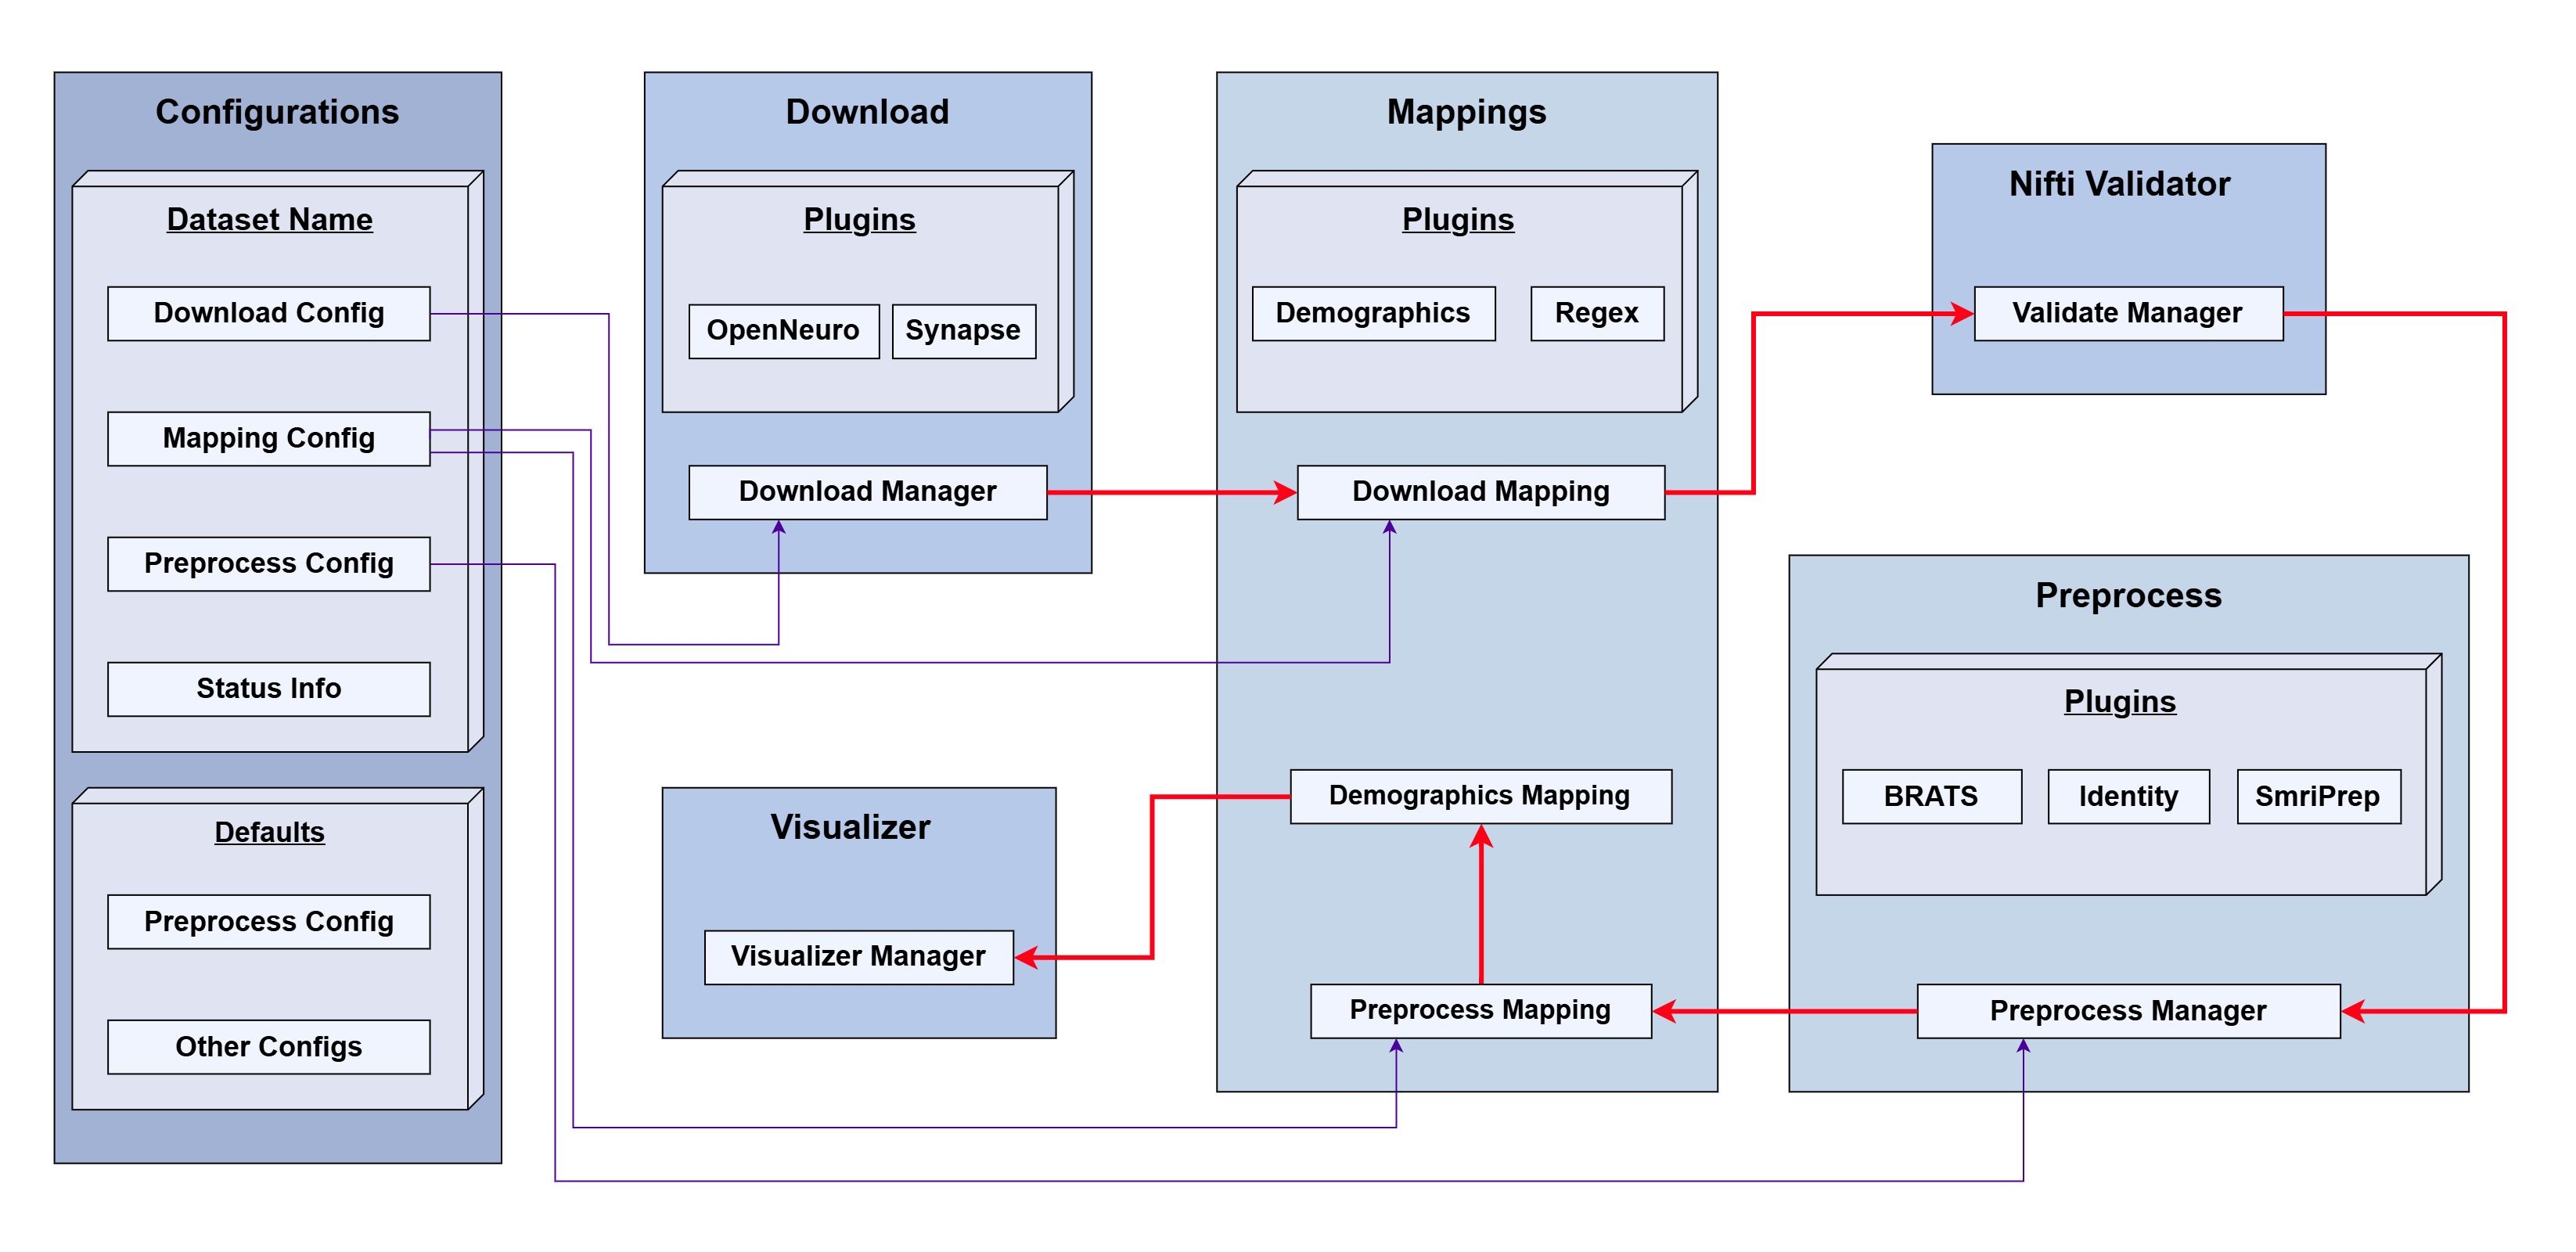
\includegraphics[width=\linewidth]{figures/architecture.png}
    \caption{
        BrainScape Framework architecture.
    }
    \label{fig:SystemArchitecture}\end{center}
\end{figure}

The pipeline workflow coordinates each module's tasks, ensuring a structured flow of data and synchronized processing. 
\textbf{Downloader Plugins}, such as the OpenNeuro downloader and Synapse downloader are used to download MRI 
data from target MRI databases and repositories.
The OpenNeuro downloader uses the \href{https://docs.aws.amazon.com/cli/latest/reference/s3/}{Amazon S3 CLI tool} to download datasets 
from OpenNeuro (\cite{markiewicz2021openneuro}) and other large-scale databases like the Human Connectome Project (HCP) (\cite{van2013wu}).
Similarly, the Synapse Downloader plugin retrieves MRI datasets from \href{https://www.synapse.org}{synapse.org}.
These plugins preserve each downloaded dataset's original folder structure, simplifying comparisons after the datasets are obtained.
\textbf{Mapper Plugins} (e.g., RegexMapper) then map the downloaded dataset files to a standardized JSON record, 
accommodating differences in dataset structure, organization, file formats, and MRI modalities based on user-defined, 
dataset-specific configuration settings.
\textbf{Validator Plugins}, such as the NIfTI Validator, check each MRI file from all of the datasets 
to detect potential errors early, thereby helping the workflow maintain high data-quality standards.
\textbf{Preprocessor Plugins} (e.g., BRATS, Identity, Smriprep) then employ preprocessing pipelines
that consist of specialized tasks, such as MRI registration, brain extraction, and intensity normalization. 
For instance, the BRATS plugin uses the \href{https://github.com/BrainLesion/preprocessing}{BrainLes-Preprocessing} tool, 
following the Brain Tumor Segmentation (BRATS) pipeline (\cite{menze2014multimodal}). 
In the BRATS pipeline, multiple MRI modalities are co-registered to a central modality (e.g., T1w), 
then mapped to the SR24 atlas (\cite{rohlfing2010sri24}), followed by skull stripping and image intensity normalization. 
Datasets already preprocessed or skull-stripped can opt for simpler pipelines, 
such as the ``Identity'' preprocessor, which applies no additional operations. 
Other preprocessing pipelines can also be introduced as needed, maintaining the flexibility and modularity.
After preprocessing, \textbf{Mapper plugins} (e.g., RegexMapper) update the standardized JSON record 
with the preprocessed MRI files. The \textbf{Demographics Mapper} plugin then appends relevant demographic 
and clinical fields (e.g., age, sex, diagnosis) to each subject record, thereby producing a unified 
resource that integrates both anatomical and demographic information.

This modular architecture supports plugin swaps via configuration files, 
eliminating the need to alter the codebase. As a result, researchers can 
readily include additional plugins supporting specialized pipelines for their unique study requirements. 
BrainScape's pipeline workflow and configurable plugins provide a robust, adaptable system for MRI data management.


\subsection{Experimental Setup and Performance Measurement}

We conducted our experiments on a local workstation equipped with a 13th Generation Intel Core i9-13900K CPU 
and an NVIDIA GeForce RTX 4070 Ti GPU (12GB VRAM). 
The CPU has 24 physical cores running at speeds of up to 5.8\,GHz. 
The pipeline was tested using Python 3.11 on Ubuntu 22.04.
To evaluate the BrainScape pipeline, 
we selected the publicly available \href{https://openneuro.org/datasets/ds003717}{VASP dataset} (\cite{peelle2022increased}) from OpenNeuro, 
which includes T1w and T2w MRI scans for 60 subjects (120 MRI scans in total). 

We utilized several Python packages to capture performance metrics: 
``time'' for measuring wall-clock time, 
\href{https://docs.python.org/3/library/resource.html}{resource} for computing CPU time,
\href{https://pypi.org/project/psutil/}{psutil} to calculate average CPU utilization, 
\href{https://pypi.org/project/pynvml/}{pynvml} for GPU usage and memory consumption, and 
\href{https://pypi.org/project/codecarbon/}{CodeCarbon} to estimate electricity consumption (kWh) and CO$_2$-equivalents (CO$_2$eq) emissions, 
using the carbon intensity data from New Zealand's local electricity grid.

Currently, the pipeline is designed to process datasets sequentially. 
Nevertheless, its modular design and configurable workflow support running multiple datasets in parallel 
which will be effective in reducing the overall wall-clock time.


